\documentclass{article}

\usepackage[utf8]{inputenc}
\usepackage{graphicx}
\usepackage{amsmath}
\usepackage[letterpaper, portrait, margin=1in]{geometry}
\usepackage{booktabs}

\title{Molecules and Cells HW 4}
\date{September 22nd, 2016}

\begin{document}

\maketitle

1a.	$n=1$ because myoglobin only has a single binding site for oxygen.

1b. Although hemoglobin has 4 binding sites, an n value of 2.8 means that the binding sites are not completely independent. The $K_d$ value of binding another oxygen would change depending on the amount of oxygen molecules already bound to hemoglobin.

1c. \begin{figure}[h]
  \centering
  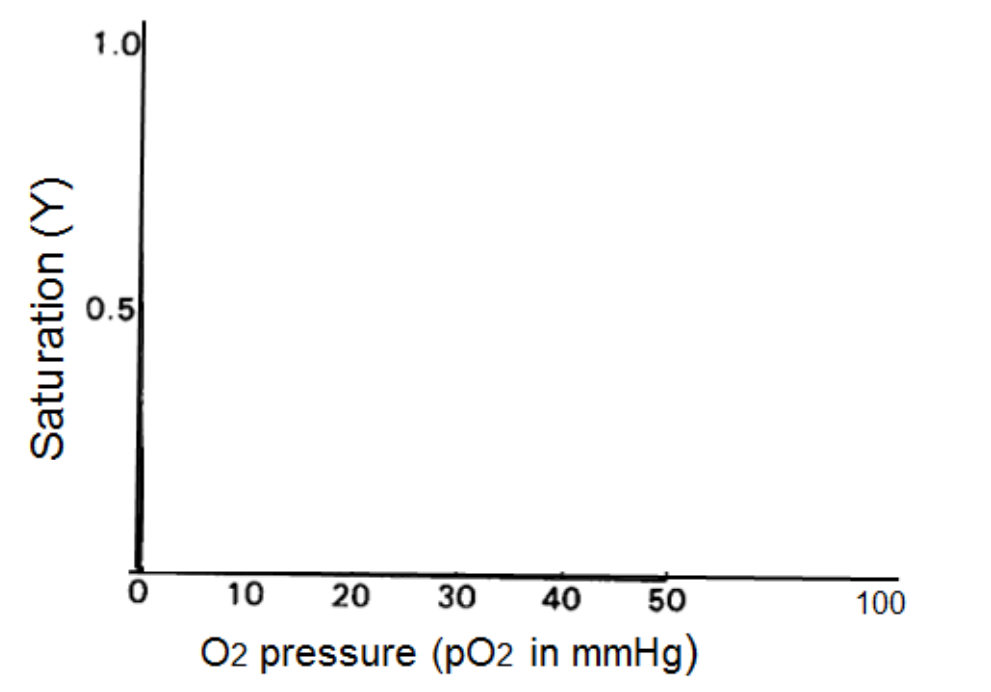
\includegraphics[scale=0.25]{PartialPressureBlank.png}
\end{figure}

1d. In the lungs, they should have the same saturation because partial pressure is high. Once they reach tissue, though, the mutant Hb would have more affinity to oxygen, leading to a lower blood oxygen saturation. As shown in the graph above

2a. $$K_d=\frac{[HbO_2][H+]^{0.7}}{[Hb][O_2]}$$

2b. The concentration would increase initially.

2c. The acidity would increase. The excess $CO_2$ would be converted to $H_2CO_3$ which produce more $H^+$ ions, resulting in a drop in pH.

2d-e. \begin{figure}[h]
  \centering
  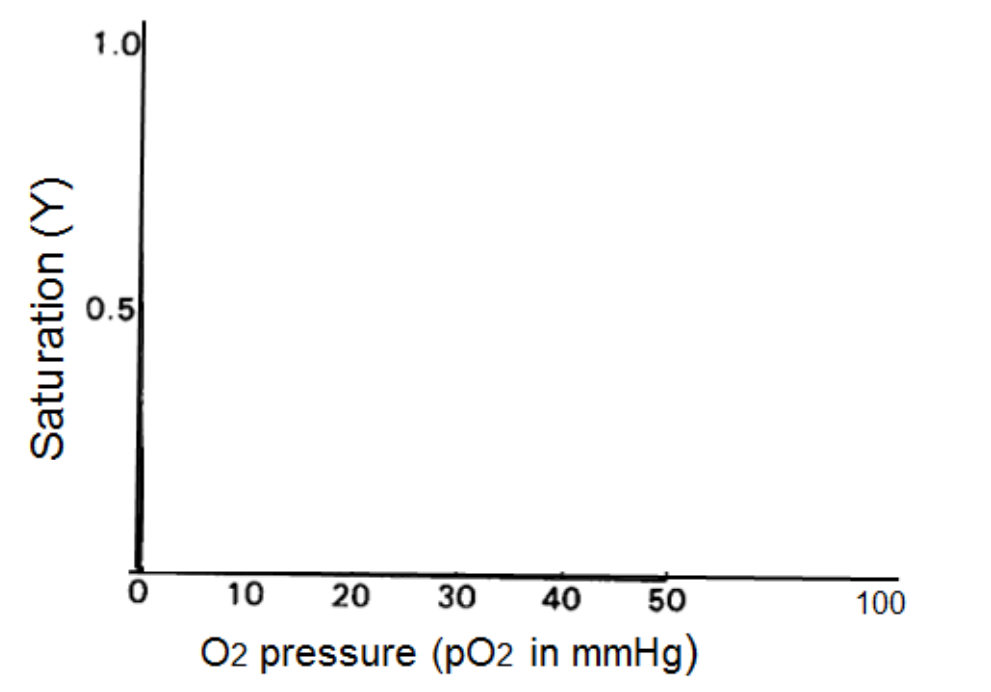
\includegraphics[scale=0.25]{PartialPressureBlank.png}
\end{figure}

2f. Since the person cannot convert $CO_2$ as well, there wouldn't be as many $H^+$ ions, so the pH would increase, resulting in a left shift compared to e.

3. (D). An increase in the amount of BPG increases the amount of Hb in the T state, resulting in a decrease in affinity and an increase in blood oxygen levels.

4a. When there is little product initially, the reverse reaction of the product joining the enzyme again can be assumed to be 0, which helps simplify the math. This is also a fundamental assumption for Michaelis-Menton enzymes.

4b. \begin{figure}[h]
  \centering
  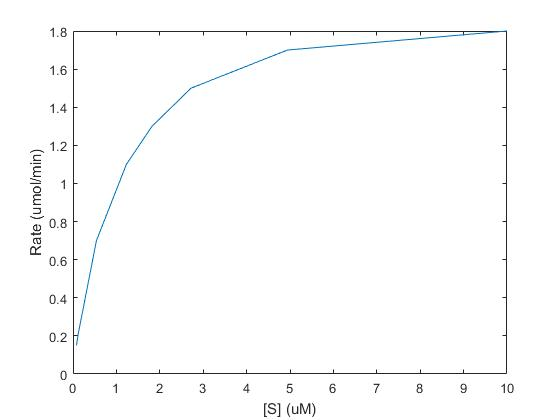
\includegraphics[scale=0.4]{michaelis-menton.jpg}
\end{figure}

The graph is the expected shape for Michaelis-Menton. By visual inspection, $V_{max}$ is about 1.8 $\mu$mol/min and $K_m$ is about 1 $\mu$M.

4c.	The Michaelis-Menton equation is 
$$V=\frac{V_{max}[S]}{K_m +[S]}$$ 
Taking the inverse of both sides gives 
$$\frac{1}{V}=\frac{K_m +[S]}{V_{max}[S]}$$ 
This can be separated into 
$$\frac{1}{V}=\frac{K_m}{V_{max}[S]}+\frac{[S]}{V_{max}[S]}
=\frac{K_m}{V_{max}}\left[\frac{1}{[S]}\right]+\frac{1}{V_{max}}$$

4d. \begin{figure}[h]
  \centering
  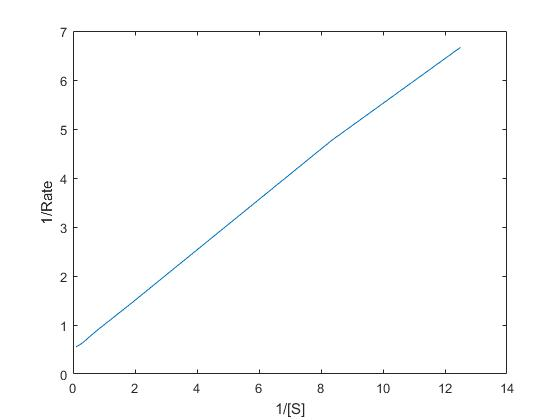
\includegraphics[scale=0.4]{lineweaver-burk.jpg}
\end{figure}

The slope is about 0.493 and the y-intercept is about 0.502. Since the y-intercept is equal to $\frac{1}{V_{max}}$, $$V_{max}=1.992$$ Then, since the slope is equal to 
$\frac{K_m}{V_{max}}$,
$$K_m=0.982$$

5. (D) Competitive inhibition would decrease $V_m$ since it would take more substrate molecules to get the same effective rate, but $V_{max}$ would stay the same. Since noncompetitive inhibition physically changes the shape of the enzyme, $V_{max}$ would decrease since those enzymes can be reacted with. In the graph below, black represents the regular enzyme, blue represents competitive inhibition, and red represents noncompetitive inhibition.

\begin{figure}[h]
  \centering
  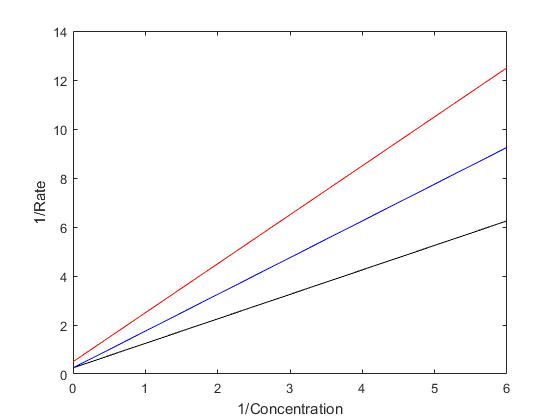
\includegraphics[scale=0.3]{P5.jpg}
\end{figure}

6a. Although individual enzymes may be active or not, not all enzymes have to be active at the same time. Therefore, depending on the number of enzymes activated, the rate can vary from completely uncatalyzed to completely catalyzed and include every rate in between.

6b. A greater $K_m$ value indicates that a greater concentration of substrate would be needed to achieve the same rate, specifically the rate of $\frac{V_{max}}{2}$. Since the rate at the given concentration decreases, phosphorylation inhibits the enzyme. 

7. The Michaelis-Menton equation is 
$$V=\frac{V_{max}[S]}{K_m +[S]}$$ 
At $0.2V_{max}$, 
$$0.2V_{max}=\frac{V_{max}[S]_{0.2}}{K_m+[S]_{0.2}},0.2=\frac{[S]_{0.2}}{K_m +[S]_{0.2}}$$ At $0.8V_{max}$,
$$0.8V_{max}=\frac{V_{max}[S]_{0.8}}{K_m +[S]_{0.8}},0.8=\frac{[S]_{0.8}}{K_M +[S]_{0.8}}$$
Solving for $K_m$ in oth equations gives 
$$K_m=\frac{[S]_{0.2}}{0.2}-[S]_{0.2}=4[S]_{0.2}$$
$$K_m=\frac{[S]_{0.8}}{0.8}-[S]_{0.8}=\frac{[S]_{0.8}}{4}$$ 
Finally, setting the two equations equal to each other gives 
$$\frac{[S]_{0.8}}{4}=4[S]_{0.2},[S]_{0.8}=16[S]_{0.2}$$

8a. $T+S\rightleftharpoons TS\rightleftharpoons T+S$

8b. Assuming that there is no reverse reaction sending the solute up the concentration gradient, the equation would be the same
$$V=\frac{V_{max}[S]}{K_m +[S]}$$ 
Where [S] is the concentration of solute

8c. No, the fundamental idea of Michaelis-Menton is that there is no reverse reaction of the product connecting to the enzyme, which would not be the case in a channel. In addition to this, since the rate of S traveling through the channel is so large, the assumption that the concentration of S will stay constant over small periods of time is also false.

9a. Dividing both sides of the Michaelis-Menton equation by $V_{max}$ gives 
$$\frac{V}{V_{max}}=\frac{[S]}{K_m +[S]}$$
Using this formula and plugging in the provided numbers gives the following

\begin{table}[h!]
  \centering
  \begin{tabular}{ccc}
    \toprule
    & Brain & Liver\\
    \midrule
    3 mM & 66.67\% & 16.67\%\\
    5 mM & 76.92\% & 25.00\%\\
    7 mM & 82.35\% & 31.82\%\\
    \bottomrule
  \end{tabular}
\end{table}

9b. Using the same formula as before with $[S]=15$ mM, $V_m=15$ mM,
$$\frac{V}{V_{max}}=0.5=50\%$$

9c. Since glucose should be stored in the liver, it makes sense that the rate would be much slower in the liver as compared to the brain cells. There should be enough glucose in the brain cells for glycolysis and energy production 

10. (C) $V_{max}$ is an intrinsic property of enzymes that cannot be changed by moving them around. All the other responses might be improved, but the only way to improve $V_{max}$ would be to add some sort of activator.

11. (E) If the protein is completely unfolded, it would not be able to react with Y, meaning the organism would not be able to turn pink.

12. (C) Because hydrophobic interactions are entropy-driven, they strengthen when entropy increases. 
\end{document}